% !TEX encoding = UTF-8 Unicode
\documentclass{beamer}

\usepackage{amsmath}
\usepackage{amssymb}

\usetheme{Warsaw}

\newcommand{\btVFill}{\vskip0pt plus 1filll}

\title[Neural temporal point processes for earthquake catalogs]{Neural temporal point processes for earthquake catalogs}
\author{Ariane Ducellier}
\institute{University of Washington}
\date{SeismoLunch - February 23\textsuperscript{rd} 2022}

\begin{document}

	\begin{frame}
		\titlepage
	\end{frame}

	\section{Point processes}
	\subsection{What is a point process?}

	\begin{frame}
		\frametitle{What is a point process?}
		A point process is a random collection of points falling in some space.

		\vspace{1em}

		For a temporal point process, the space is a portion of the real line.

		\vspace{1em}

		$\rightarrow$ Ex: A collection of timings of earthquake events.

		\vspace{2em}

		For a marked point process, there is also some information associated with the timing of the events.

		\vspace{1em}

		$\rightarrow$ Ex: A collection of timings and magnitudes of earthquake events.
	\end{frame}

	\subsection{Conditional intensity function (CIF)}

	\begin{frame}
		\frametitle{Conditional intensity function (CIF)}
		$N_{\delta} \left( t \right)$: Number of events between $t$ and $t + \delta$.

		\vspace{1em}

		$\mathcal{H}_t =  \left\{ (\left( t_i , m_i \right) \forall i : t_i < t \right\} $: Event history up to time $t$.

		\vspace{2em}

		Conditional intensity function ($\sim$ event rate):

		\vspace{1em}

		$\lambda \left( t \mid \mathcal{H}_t \right) = \lim_{\delta \rightarrow 0} Pr \left\{ N_{\delta} \left( t \right) > 0 \mid \mathcal{H}_t \right\}$

		\vspace{2em}

		Our objective: Computing the value of $\lambda \left( t \right)$ knowing the event sequence $\left\{ \left(t_1 , m_1 \right) , \cdots , \left( t_n , m_n \right) \right\}$ between $T_1$ and $T_2$.
	\end{frame}

	\section{ETAS model}
	\subsection{Epidemic-Type Aftershock Sequence model}

	\begin{frame}
		\frametitle{Epidemic-Type Aftershock Sequence (ETAS) model}
		\begin{itemize}
			\item Magnitude-frequency distribution law of Gutenberg and Richter: $Pr \left( m_i > m \right) = e^{- \beta \left( m - m_C \right)} \text{ for } m > m_C$.
			\item Omori-Utsu law of aftershock decay: Number of aftershocks decays as $1 / t^p$.
			\item Each event, irrespective of whether it is a small or a big event, can trigger its own offspring.
		\end{itemize}

		\begin{equation*}
		\lambda \left( t \mid \mathcal{H}_t \right) = \mu + \sum_{i : t_i < t} A e^{\alpha \left( m_i - m_C \right)} \left( 1 + \frac{t - t_i}{c} \right) ^{-p}
		\end{equation*}		
	\end{frame}

	\subsection{Fitting an ETAS model}

	\begin{frame}
		\frametitle{Fitting an ETAS model}
		Find the parameters $\left( \mu , A , \alpha , c , p \right)$ that maximizes the likelihood:

		\begin{equation*}
		\begin{aligned}
		L = & Pr \left\{ \text{The first event occurs between } t_1 \text{ and } t_1 + dt \mid \right. \\
		& \left. \mathcal{H}_{T_1} \text{ and the first event does not occur between } T_1 \text{ and } t_1 \right\} * \\
		& Pr \left\{ \text{The second event occurs between } t_2 \text{ and } t_2 + dt \mid \right. \\
		& \left. \mathcal{H}_{t_1} \text{ and the second event does not occur between } t_1 \text{ and } t_2 \right\} * \\
		& \cdots \\
		& Pr \left\{ \text{The last event occurs between } t_n \text{ and } t_n + dt \mid \right. \\
		& \left. \mathcal{H}_{t_{n - 1}} \text{ and the last event does not occur between } t_{n - 1} \text{ and } t_n \right\}
		\end{aligned}
    		\end{equation*}
	\end{frame}

	\begin{frame}
		\frametitle{Fitting an ETAS model}
		Find the parameters $\left( \mu , A , \alpha , c , p \right)$ that maximizes the log-likelihood:

		\begin{equation*}
		l = \sum_{i : T_1 \leq t_i \leq T_2} \log \lambda \left( t \mid \mathcal{H}_{t_i} \right) - \int_{T_1}^{T_2} \lambda \left( t \mid \mathcal{H}_t \right) dt
    		\end{equation*}
	\end{frame}

	\subsection{Goodness of fit}

	\begin{frame}
		\frametitle{Goodness of fit of ETAS model}
		Residual process:

		\vspace{1em}

		Transform times $\tau_i = \int_{T_1}^{t_i} \hat{\lambda} \left( t \mid \mathcal{H}_t \right) dt$ where $\hat{\lambda}$ is the fitted conditional intensity function.

		\vspace{2em}

		Plot $\tau_i$ as a function of $i$. There is a good fit if the points follow the straight line $y = x$.

		\vspace{1em}

		Plot $\tau_i - i$ as a function of $i$. There is a good fit if the points are horizontally aligned.
	\end{frame}

	\subsection{Results}

	\begin{frame}
		\frametitle{Example on an LFE family using R package PtProcess}
		\vspace{1em}
		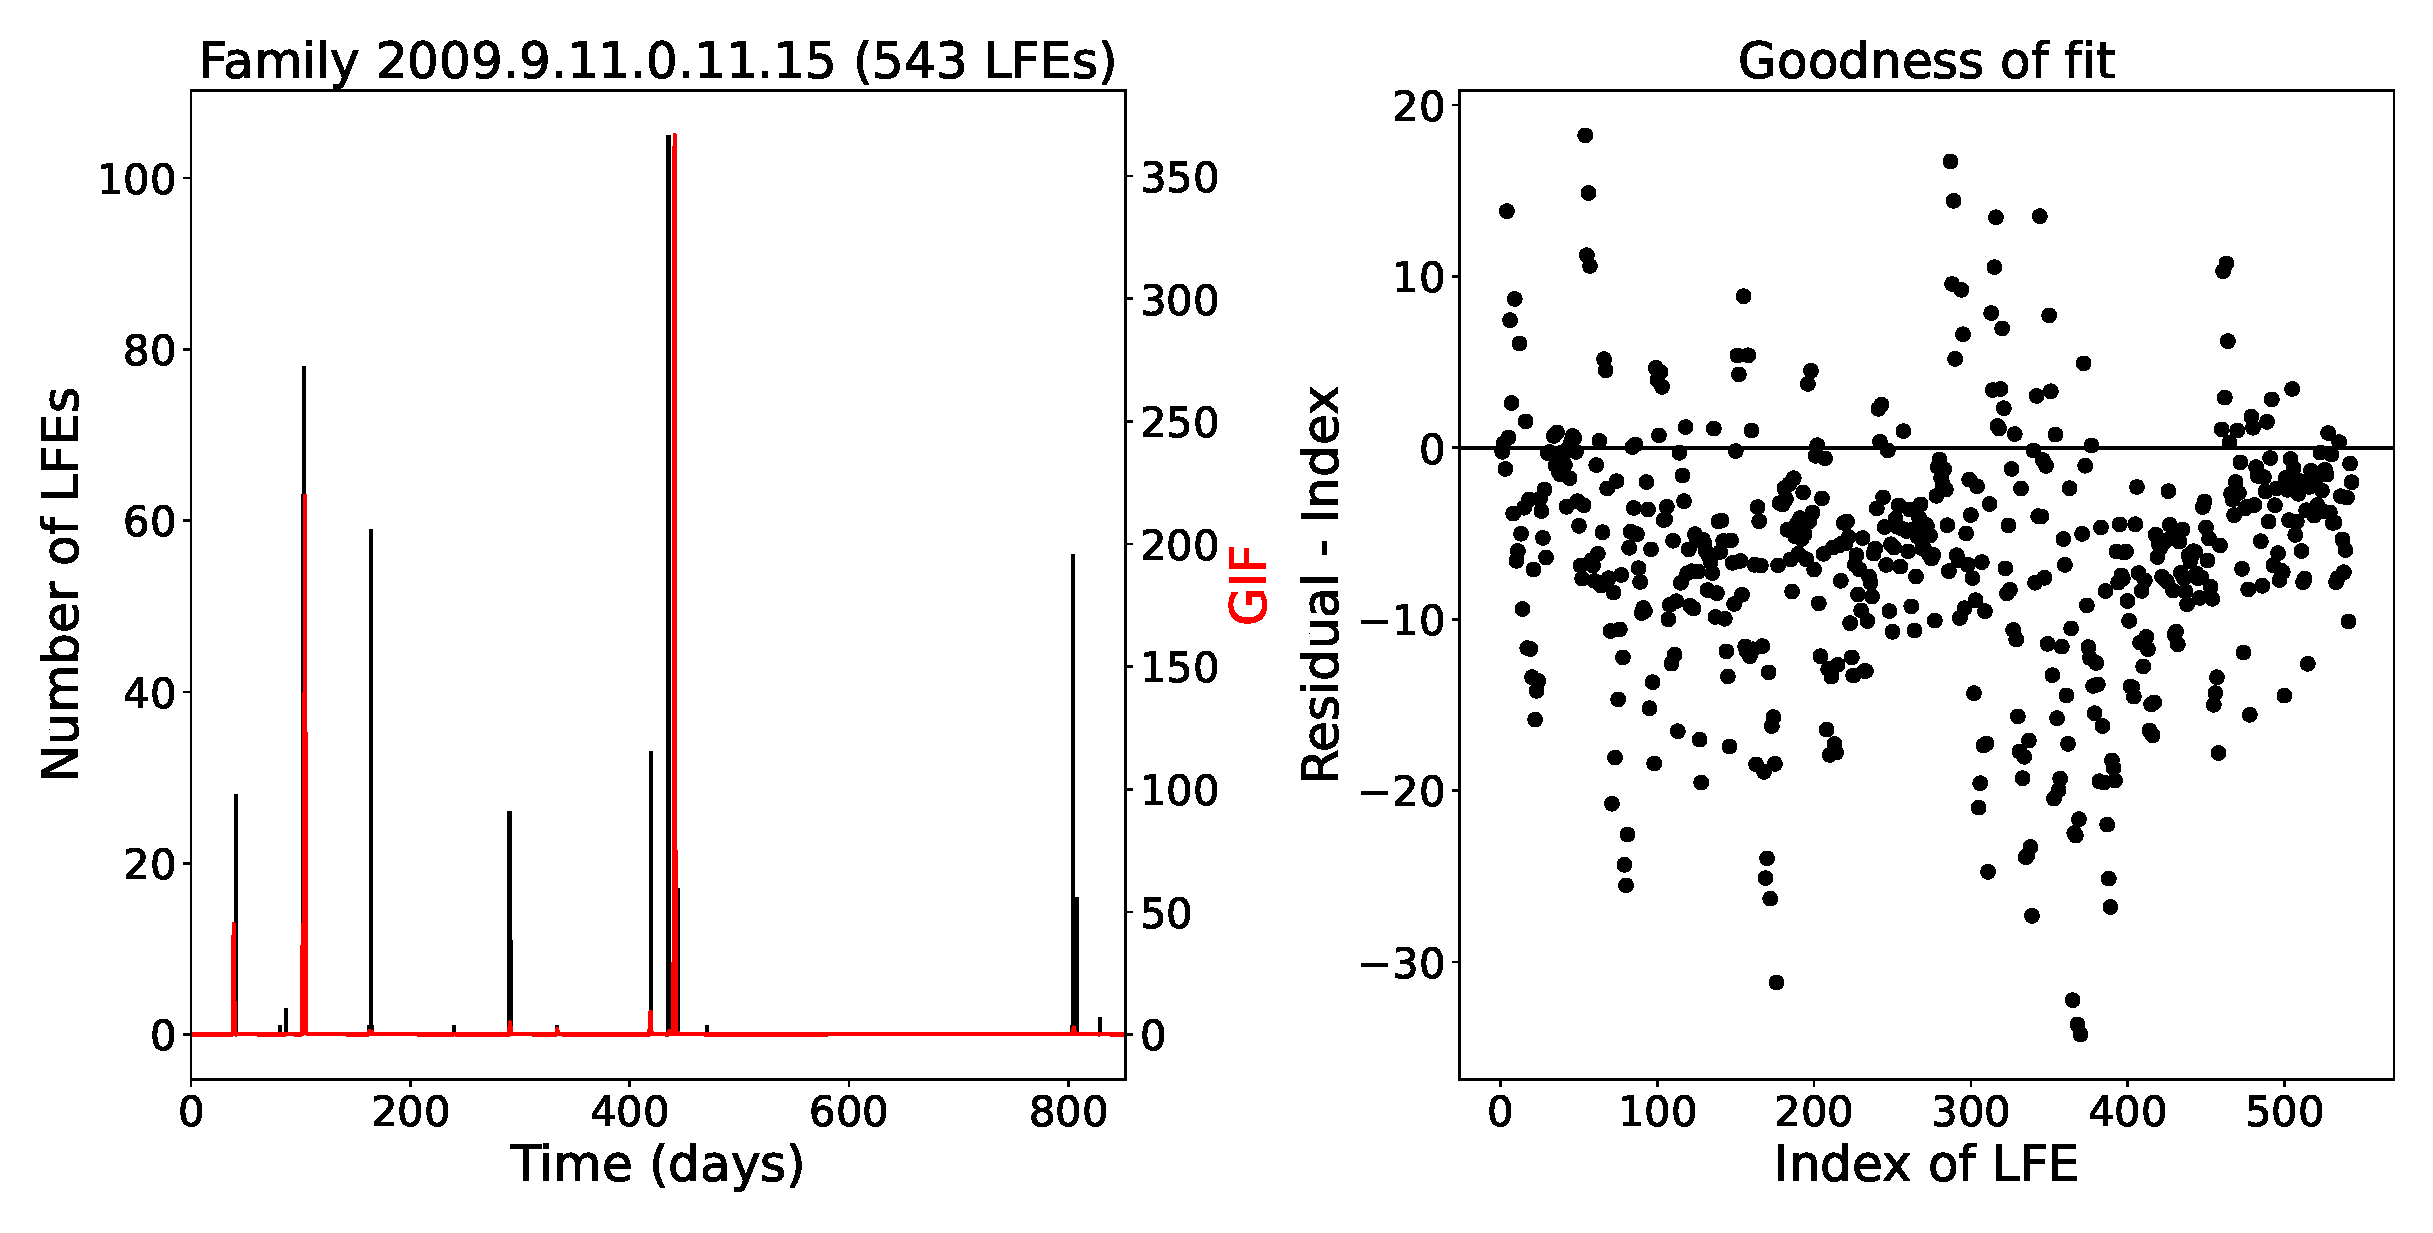
\includegraphics[trim={0cm 0cm 0cm 0cm}, clip, width=11cm]{gif_residuals_PtProcess.eps}
		\btVFill
		\tiny{LFE catalog from Chestler and Creager (2017).}
	\end{frame}

	\section{Neural networks for point processes}

	\begin{frame}
		\frametitle{More about ETAS and NTPP}
		\begin{itemize}
			\item CORSSA
			\item Technical session at SSA meeting: New Developments in Physics- and Statistics-based Earthquake Forecasting oral session (Friday 10am to 11:15 am)
			\item Olksandr Shchur blog
		\end{itemize}
	\end{frame}
		
	\begin{frame}
		\begin{Huge}
			\begin{center}
				Questions?
			\end{center}
		\end{Huge}
	\end{frame}
			
\end{document}
